%\documentclass[12p,preprint]{elsarticle}
\documentclass[3p]{elsarticle}

\usepackage{amssymb}
\usepackage{moreverb}
\usepackage{empheq}
\usepackage{amssymb,bm,amsbsy,graphicx,color,amsmath,amsfonts}
\usepackage{mathrsfs}
\usepackage{latexsym}
\usepackage{pseudocode}
\usepackage{epsfig,epsf,rotating}
\usepackage{subfig}
\usepackage{epstopdf}
\usepackage{framed}
\usepackage[dvipsnames]{xcolor}
\usepackage{alltt}
\usepackage{lipsum}
\usepackage{mathrsfs}
\usepackage{tikz}
\usepackage{xcolor}
\usepackage{framed}
\DeclareMathAlphabet{\mathscrbf}{OMS}{mdugm}{b}{n}

\biboptions{sort&compress}

%\newcommand{\vect}[1]{\boldsymbol{#1}}
%\DeclareMathOperator{\tr}{tr}
%% Loads stmaryrd symbols for 10pt plain TeX documents.
% Use \stmaryrdninepoint for nine point documents.
% Use \stmaryrdelevenpoint for eleven point documents.
% Use \stmaryrdtwelvepoint for twelve point documents.
%
% See stmaryrd docs for the symbols available and the commands to
% access them.

\edef\restoreallcatcodes{%
   \catcode`\noexpand\@=\number\catcode`\@\relax
   \catcode`\noexpand\!=\number\catcode`\!\relax}

\newfam\stmaryrdfam

\font\stmaryfiv  stmary5
\font\stmarysix  stmary6
\font\stmarysev  stmary7
\font\stmaryegt  stmary8
\font\stmarynin  stmary9
\font\stmaryten  stmary10
\font\stmaryelv  stmary10 at10.95pt
\font\stmarytwl  stmary10 at12pt

\def\stmaryrdninepoint{%
  \textfont\stmaryrdfam\stmarynin
  \scriptfont\stmaryrdfam\stmarysev
  \scriptscriptfont\stmaryrdfam\stmaryfiv}

\def\stmaryrdtenpoint{%
  \textfont\stmaryrdfam\stmaryten
  \scriptfont\stmaryrdfam\stmarysev
  \scriptscriptfont\stmaryrdfam\stmaryfiv}

\def\stmaryrdelevenpoint{%
  \textfont\stmaryrdfam\stmaryelv
  \scriptfont\stmaryrdfam\stmarysegt
  \scriptscriptfont\stmaryrdfam\stmarysix}

\def\stmaryrdtwelvepoint{%
  \textfont\stmaryrdfam\stmarytwl
  \scriptfont\stmaryrdfam\stmaryegt
  \scriptscriptfont\stmaryrdfam\stmarysix}

\catcode`\@=11
\def\hexnumber@#1{\ifcase#1%
  0\or 1\or 2\or 3\or 4\or 5\or 6\or 7\or
  8\or 9\or A\or B\or C\or D\or E\or F\fi}

\catcode`\!\active
\edef!{\hexnumber@\stmaryrdfam}

\mathchardef\shortleftarrow"3!00
\mathchardef\shortrightarrow"3!01
\mathchardef\shortuparrow"3!02
\mathchardef\shortdownarrow"3!03
\mathchardef\Yup"2!04
\mathchardef\Ydown"2!05
\mathchardef\Yleft"2!06
\mathchardef\Yright"2!07
\mathchardef\varcurlyvee"2!08
\mathchardef\varcurlywedge"2!09
\mathchardef\minuso"2!0A
\mathchardef\baro"2!0B
\mathchardef\sslash"2!0C
\mathchardef\bbslash"2!0D
\mathchardef\moo"2!0E
\mathchardef\varotimes"2!0F
\mathchardef\varoast"2!10
\mathchardef\varobar"2!11
\mathchardef\varodot"2!12
\mathchardef\varoslash"2!13
\mathchardef\varobslash"2!14
\mathchardef\varocircle"2!15
\mathchardef\varoplus"2!16
\mathchardef\varominus"2!17
\mathchardef\boxast"2!18
\mathchardef\boxbar"2!19
\mathchardef\boxdot"2!1A
\mathchardef\boxslash"2!1B
\mathchardef\boxbslash"2!1C
\mathchardef\boxcircle"2!1D
\mathchardef\boxbox"2!1E
\mathchardef\boxempty"2!1F
\mathchardef\lightning"0!20
\mathchardef\merge"2!21
\mathchardef\vartimes"2!22
\mathchardef\fatsemi"2!23
\mathchardef\sswarrow"3!24
\mathchardef\ssearrow"3!25
\mathchardef\curlywedgeuparrow"3!26
\mathchardef\curlywedgedownarrow"3!27
\mathchardef\fatslash"2!28
\mathchardef\fatbslash"2!29
\mathchardef\lbag"2!2A
\mathchardef\rbag"2!2B
\mathchardef\varbigcirc"2!2C
\mathchardef\leftrightarroweq"3!2D
\mathchardef\curlyveedownarrow"3!2E
\mathchardef\curlyveeuparrow"3!2F
\mathchardef\nnwarrow"3!30
\mathchardef\nnearrow"3!31
\mathchardef\leftslice"2!32
\mathchardef\rightslice"2!33
\mathchardef\varolessthan"2!34
\mathchardef\varogreaterthan"2!35
\mathchardef\varovee"2!36
\mathchardef\varowedge"2!37
\mathchardef\talloblong"2!38
\mathchardef\interleave"2!39
\mathchardef\obar"2!3A
\mathchardef\obslash"2!3B
\mathchardef\olessthan"2!3C
\mathchardef\ogreaterthan"2!3D
\mathchardef\ovee"2!3E
\mathchardef\owedge"2!3F
\mathchardef\oblong"2!40
\mathchardef\inplus"3!41
\mathchardef\niplus"3!42
\mathchardef\nplus"2!43
\mathchardef\subsetplus"3!44
\mathchardef\supsetplus"3!45
\mathchardef\subsetpluseq"3!46
\mathchardef\supsetpluseq"3!47
\mathchardef\Lbag"4!48
\mathchardef\Rbag"5!49

\mathchardef\llparenthesis"4!4C
\mathchardef\rrparenthesis"5!4D
\mathchardef\binampersand"4!4E
\mathchardef\bindnasrepma"5!4F
\mathchardef\trianglelefteqslant"3!50
\mathchardef\trianglerighteqslant"3!51
\mathchardef\ntrianglelefteqslant"3!52
\mathchardef\ntrianglerighteqslant"3!53
\mathchardef\llfloor"4!54
\mathchardef\rrfloor"5!55
\mathchardef\llceil"4!56
\mathchardef\rrceil"5!57
\mathchardef\arrownot"3!58
\mathchardef\Arrownot"3!59
\mathchardef\Mapstochar"3!5A
\mathchardef\mapsfromchar"3!5B
\mathchardef\Mapsfromchar"3!5C
\mathchardef\leftrightarrowtriangle"2!5D
\mathchardef\leftarrowtriangle"3!5E
\mathchardef\rightarrowtriangle"3!5F
\mathchardef\bigtriangledown"1!60
\mathchardef\bigtriangleup"1!61
\mathchardef\bigcurlyvee"1!62
\mathchardef\bigcurlywedge"1!63
\mathchardef\bigsqcap"1!64
\mathchardef\bigbox"1!65
\mathchardef\bigparallel"1!66
\mathchardef\biginterleave"1!67
\mathchardef\bignplus"1!70

\edef\llbracket{\delimiter"4!4A!71}
\edef\rrbracket{\delimiter"5!4B!79}

\def\@tempa#1{
  \def\varcopyright{{\ooalign{\hfil\raise.07ex\hbox{c}\hfil\crcr\mathhexbox#12C}}}}
\expandafter\@tempa!

% The long arrow negations.

\def\longarrownot{\mathrel{\mkern5.5mu\arrownot\mkern-5.5mu}}
\def\Longarrownot{\mathrel{\mkern5.5mu\Arrownot\mkern-5.5mu}}

% The variants on \mapsto:

\def\Mapsto{\Mapstochar\Rightarrow}
\def\mapsfrom{\leftarrow\mapsfromchar}
\def\Mapsfrom{\Leftarrow\Mapsfromchar}
\def\Longmapsto{\Mapstochar\Longrightarrow}
\def\longmapsfrom{\longleftarrow\mapsfromchar}
\def\Longmapsfrom{\Longleftarrow\Mapsfromchar}

\restoreallcatcodes

\stmaryrdtenpoint
 % include jump condition
%\graphicspath{{../../../0.figures/}}
%\usepackage[colorlinks,bookmarksopen,bookmarksnumbered,citecolor=red,urlcolor=red]{hyperref}

\newcommand{\boxalign}[2][0.97\textwidth]{
	\par\noindent\tikzstyle{mybox} = [draw=black,very thick,inner sep=6pt]
	\begin{center}\begin{tikzpicture}
		\node [mybox] (box){%
			\begin{minipage}{#1}{\vspace{-5mm}#2}\end{minipage}
		};
		\end{tikzpicture}\end{center}
}

\newcommand{\vect}[1]{\boldsymbol{#1}}
\newcommand{\txtbld}[1]{\text{\textbf{#1}}}
\newcommand{\cof}{\mathop{\mathrm{cof}}}
\newcommand{\addcitation}{\textcolor{red}{(citation)}}
% Loads stmaryrd symbols for 10pt plain TeX documents.
% Use \stmaryrdninepoint for nine point documents.
% Use \stmaryrdelevenpoint for eleven point documents.
% Use \stmaryrdtwelvepoint for twelve point documents.
%
% See stmaryrd docs for the symbols available and the commands to
% access them.

\edef\restoreallcatcodes{%
   \catcode`\noexpand\@=\number\catcode`\@\relax
   \catcode`\noexpand\!=\number\catcode`\!\relax}

\newfam\stmaryrdfam

\font\stmaryfiv  stmary5
\font\stmarysix  stmary6
\font\stmarysev  stmary7
\font\stmaryegt  stmary8
\font\stmarynin  stmary9
\font\stmaryten  stmary10
\font\stmaryelv  stmary10 at10.95pt
\font\stmarytwl  stmary10 at12pt

\def\stmaryrdninepoint{%
  \textfont\stmaryrdfam\stmarynin
  \scriptfont\stmaryrdfam\stmarysev
  \scriptscriptfont\stmaryrdfam\stmaryfiv}

\def\stmaryrdtenpoint{%
  \textfont\stmaryrdfam\stmaryten
  \scriptfont\stmaryrdfam\stmarysev
  \scriptscriptfont\stmaryrdfam\stmaryfiv}

\def\stmaryrdelevenpoint{%
  \textfont\stmaryrdfam\stmaryelv
  \scriptfont\stmaryrdfam\stmarysegt
  \scriptscriptfont\stmaryrdfam\stmarysix}

\def\stmaryrdtwelvepoint{%
  \textfont\stmaryrdfam\stmarytwl
  \scriptfont\stmaryrdfam\stmaryegt
  \scriptscriptfont\stmaryrdfam\stmarysix}

\catcode`\@=11
\def\hexnumber@#1{\ifcase#1%
  0\or 1\or 2\or 3\or 4\or 5\or 6\or 7\or
  8\or 9\or A\or B\or C\or D\or E\or F\fi}

\catcode`\!\active
\edef!{\hexnumber@\stmaryrdfam}

\mathchardef\shortleftarrow"3!00
\mathchardef\shortrightarrow"3!01
\mathchardef\shortuparrow"3!02
\mathchardef\shortdownarrow"3!03
\mathchardef\Yup"2!04
\mathchardef\Ydown"2!05
\mathchardef\Yleft"2!06
\mathchardef\Yright"2!07
\mathchardef\varcurlyvee"2!08
\mathchardef\varcurlywedge"2!09
\mathchardef\minuso"2!0A
\mathchardef\baro"2!0B
\mathchardef\sslash"2!0C
\mathchardef\bbslash"2!0D
\mathchardef\moo"2!0E
\mathchardef\varotimes"2!0F
\mathchardef\varoast"2!10
\mathchardef\varobar"2!11
\mathchardef\varodot"2!12
\mathchardef\varoslash"2!13
\mathchardef\varobslash"2!14
\mathchardef\varocircle"2!15
\mathchardef\varoplus"2!16
\mathchardef\varominus"2!17
\mathchardef\boxast"2!18
\mathchardef\boxbar"2!19
\mathchardef\boxdot"2!1A
\mathchardef\boxslash"2!1B
\mathchardef\boxbslash"2!1C
\mathchardef\boxcircle"2!1D
\mathchardef\boxbox"2!1E
\mathchardef\boxempty"2!1F
\mathchardef\lightning"0!20
\mathchardef\merge"2!21
\mathchardef\vartimes"2!22
\mathchardef\fatsemi"2!23
\mathchardef\sswarrow"3!24
\mathchardef\ssearrow"3!25
\mathchardef\curlywedgeuparrow"3!26
\mathchardef\curlywedgedownarrow"3!27
\mathchardef\fatslash"2!28
\mathchardef\fatbslash"2!29
\mathchardef\lbag"2!2A
\mathchardef\rbag"2!2B
\mathchardef\varbigcirc"2!2C
\mathchardef\leftrightarroweq"3!2D
\mathchardef\curlyveedownarrow"3!2E
\mathchardef\curlyveeuparrow"3!2F
\mathchardef\nnwarrow"3!30
\mathchardef\nnearrow"3!31
\mathchardef\leftslice"2!32
\mathchardef\rightslice"2!33
\mathchardef\varolessthan"2!34
\mathchardef\varogreaterthan"2!35
\mathchardef\varovee"2!36
\mathchardef\varowedge"2!37
\mathchardef\talloblong"2!38
\mathchardef\interleave"2!39
\mathchardef\obar"2!3A
\mathchardef\obslash"2!3B
\mathchardef\olessthan"2!3C
\mathchardef\ogreaterthan"2!3D
\mathchardef\ovee"2!3E
\mathchardef\owedge"2!3F
\mathchardef\oblong"2!40
\mathchardef\inplus"3!41
\mathchardef\niplus"3!42
\mathchardef\nplus"2!43
\mathchardef\subsetplus"3!44
\mathchardef\supsetplus"3!45
\mathchardef\subsetpluseq"3!46
\mathchardef\supsetpluseq"3!47
\mathchardef\Lbag"4!48
\mathchardef\Rbag"5!49

\mathchardef\llparenthesis"4!4C
\mathchardef\rrparenthesis"5!4D
\mathchardef\binampersand"4!4E
\mathchardef\bindnasrepma"5!4F
\mathchardef\trianglelefteqslant"3!50
\mathchardef\trianglerighteqslant"3!51
\mathchardef\ntrianglelefteqslant"3!52
\mathchardef\ntrianglerighteqslant"3!53
\mathchardef\llfloor"4!54
\mathchardef\rrfloor"5!55
\mathchardef\llceil"4!56
\mathchardef\rrceil"5!57
\mathchardef\arrownot"3!58
\mathchardef\Arrownot"3!59
\mathchardef\Mapstochar"3!5A
\mathchardef\mapsfromchar"3!5B
\mathchardef\Mapsfromchar"3!5C
\mathchardef\leftrightarrowtriangle"2!5D
\mathchardef\leftarrowtriangle"3!5E
\mathchardef\rightarrowtriangle"3!5F
\mathchardef\bigtriangledown"1!60
\mathchardef\bigtriangleup"1!61
\mathchardef\bigcurlyvee"1!62
\mathchardef\bigcurlywedge"1!63
\mathchardef\bigsqcap"1!64
\mathchardef\bigbox"1!65
\mathchardef\bigparallel"1!66
\mathchardef\biginterleave"1!67
\mathchardef\bignplus"1!70

\edef\llbracket{\delimiter"4!4A!71}
\edef\rrbracket{\delimiter"5!4B!79}

\def\@tempa#1{
  \def\varcopyright{{\ooalign{\hfil\raise.07ex\hbox{c}\hfil\crcr\mathhexbox#12C}}}}
\expandafter\@tempa!

% The long arrow negations.

\def\longarrownot{\mathrel{\mkern5.5mu\arrownot\mkern-5.5mu}}
\def\Longarrownot{\mathrel{\mkern5.5mu\Arrownot\mkern-5.5mu}}

% The variants on \mapsto:

\def\Mapsto{\Mapstochar\Rightarrow}
\def\mapsfrom{\leftarrow\mapsfromchar}
\def\Mapsfrom{\Leftarrow\Mapsfromchar}
\def\Longmapsto{\Mapstochar\Longrightarrow}
\def\longmapsfrom{\longleftarrow\mapsfromchar}
\def\Longmapsfrom{\Longleftarrow\Mapsfromchar}

\restoreallcatcodes

\stmaryrdtenpoint
 % include jump condition
\usepackage[colorlinks,bookmarksopen,bookmarksnumbered,citecolor=red,urlcolor=red]{hyperref}
\DeclareMathOperator{\tr}{tr}
\DeclareMathOperator{\vmesh}{\textcolor{red}{\hat{\vect{v}}}}
%\DeclareMathOperator{\vmeshh}{\hat{\boldsymbol{v}}^h}
\newcommand{\vmeshh}{\mathop{\hat{\vect{v}}^h}}
\DeclareMathOperator{\divergence}{div}
\DeclareMathOperator{\nodu}{\vect{U}}
\DeclareMathOperator{\nodv}{\dot{\vect{U}}}
\DeclareMathOperator{\noda}{\ddot{\vect{U}}}
\DeclareMathOperator{\nodp}{\vect{P}}
\DeclareMathOperator{\nodpd}{\dot{\vect{P}}}
\DeclareMathOperator{\lres}{\mathscrbf{L}}
\newdefinition{rmk}{Remark}

\journal{xxxx}

\begin{document}

%\begin{frontmatter}

%\title{A consistent penalty formulation for 2D corotational beam to surface contact using a smooth signed distance function and a narrow band mesh}
%
%\author{author 1} \author{author 2} \author{author 3} 
%%\author{Chun Hean Lee} \author{Antonio J. Gil\corref{cor1}} \author{Javier Bonet\corref{cor2}}
%%\cortext[cor1]{Corresponding author: a.j.gil@swansea.ac.uk}
%%\cortext[cor2]{Corresponding author: j.bonet@swansea.ac.uk}
%\address{xxxx}
%
%\begin{abstract}
%
%bla bla
%
%\end{abstract}
%
%\begin{keyword}
%keyword 1 \sep keyword 2  \sep keyword 3  
%\end{keyword}

%\end{frontmatter}



%%%%%%%%%%%%%%%%%%%%%%%%%%%%%%%%%%%%%%%%%%%%%%%%%%%%%%%%%%%%%%%%%%%%%
%%%%%%%%%% Introduction%%%%%%%%%%%%%%%%%%%%%%%%%%%%%%%%%%%%%%%
\section{Introduction}
Implementation of the stick-slip "Hybrid method" as proposed in \cite{Geilinger2020}

\section{Kinematics}
\subsection{Brief overview of the corotational formulation and finite element implementation}
The derivations of the co-rotational formulation are described in \cite{Aguirre2020} (see Figure \ref{fig:corotational-config} for details). We will just summarize the important parts. We start by defining the global displacement and rotations $\vect{d}$ and their variation $\delta\vect{d}$ as
\begin{align}
	\vect{d}=\left[\begin{array}{cccc}\vect{u}_1^T&\vect{\theta}_1^T&\vect{u}_2^T&\vect{\theta}_2^T
	\end{array}\right]^T;\quad\delta\vect{d}=\left[\begin{array}{cccc}\delta\vect{u}_1^T&\delta\vect{w}_1^T&\delta\vect{u}_2^T&\delta\vect{w}_2^T
	\end{array}\right]^T.\label{eq:d-deltad}
\end{align}
\noindent Additionally, we define set of local nodal quantities and their variation, as required by the corotational formulation, as
\begin{align}
	\bar{\vect{\mathcal{D}}}=\left[\begin{array}{ccc}\bar{u}&\bar{\vect{\Theta}}_1^T&\bar{\vect{\Theta}}_2^T
	\end{array}\right]^T;\quad \delta\bar{\vect{\mathcal{D}}}=\left[\begin{array}{ccc}\delta\bar{u}&\delta\bar{\vect{\Theta}}_1^T&\delta\bar{\vect{\Theta}}_2^T
	\end{array}\right]^T.\label{eq:dbar-deltadbar}
\end{align}
Using the above definitions and finite element interpolation, the centerline displacement in the current configuration is given by 
\begin{align}
	{\vect{u}}_0^h(\xi)&=\vect{u}_1 N_1(\xi)  + \vect{u}_2 N_2(\xi) +\vect{R}_e{\vect{u}}^t(\xi).\label{eq:uoh}
\end{align}
\noindent with $\vect{R}_e$ being the rigid body rotation of the beam axes and ${\vect{u}}^t$ the transversal displacement of the beam centerline, defined as
\begin{align}
\vect{u}^t(\xi)=\left[\begin{array}{c}
		0\\
		{u}_2(\xi) \\
		{u}_3(\xi) 
	\end{array}\right]=\vect{P}_1(\xi)\left[\begin{array}{c}
		\bar{\vect{\Theta}}_1\\
		\bar{\vect{\Theta}}_2
	\end{array}\right].
\end{align}
Overall, this allows defining the variation of the centerline displacement, as well as its first and second time derivatives
\begin{align}
	\delta\vect{u}_0^h &= \vect{R}_e\vect{H}_1\vect{E}^T\delta\vect{d},\label{eq:delta-u0h}\\
	\dot{\vect{u}}_0^h &= \vect{R}_e\vect{H}_1\vect{E}^T\dot{\vect{d}},\label{eq:u0hdot-intro}\\
	\ddot{\vect{u}}_0^h &= \vect{R}_e\vect{H}_1\vect{E}^T\ddot{\vect{d}}+\vect{R}_e\vect{C}_1\vect{E}^T\dot{\vect{d}}.\label{eq:u0hddot-intro}
\end{align}
\noindent And same for the rotational variables, i.e.
\begin{align}
	\delta\vect{w}_0^h&=\vect{R}_e\vect{H}_2\vect{E}^T\delta\vect{d}\label{eq:delta-w0h},\\
	\dot{\vect{w}}_0^h&=\vect{R}_e\vect{H}_2\vect{E}^T\dot{\vect{d}},\label{eq:dotw-intro}\\
	\ddot{\vect{w}}_0^h&=\vect{R}_e\vect{H}_2\vect{E}^T\ddot{\vect{d}}+\vect{R}_e\vect{C}_2\vect{E}^T\dot{\vect{d}}.\label{eq:ddotw-intro}
\end{align}

Upon assembly, this yields the following system of equations:
\begin{align}
	\textrm{\textbf{R}}(\textrm{\textbf{D}},\dot{\textrm{\textbf{D}}},\ddot{\textrm{\textbf{D}}},t) &= \textrm{\textbf{T}}_{int}(\textrm{\textbf{D}},t) + \textrm{\textbf{T}}_k(\textrm{\textbf{D}},\dot{\textrm{\textbf{D}}},\ddot{\textrm{\textbf{D}}},t) -  \textrm{\textbf{T}}_c(\textrm{\textbf{D}},\dot{\textrm{\textbf{D}}},t) - \textrm{\textbf{F}}_{ext}(\textrm{\textbf{D}},t)=\vect{0}\label{eq:discrete-residual}
\end{align}

Solution is carried out by means of the HHT-$\alpha$ method, yielding
\begin{align}
	\textrm{\textbf{R}}^{n+\alpha}&=(1+\alpha)(\textrm{\textbf{T}}_{int}^{n+1}-\textrm{\textbf{T}}_{c}^{n+1}-\textrm{\textbf{F}}_{ext}^{n+1})-\alpha(\textrm{\textbf{T}}_{int}^{n}-\textrm{\textbf{T}}_{c}^{n}-\textrm{\textbf{F}}_{ext}^{n})+\textrm{\textbf{T}}_{k}^{n+1}=\vect{0},\label{eq:Rnalpha}\\
	\tilde{\textrm{\textbf{K}}}\Delta\textrm{\textbf{D}} &= -\textrm{\textbf{R}}^{n+\alpha},\label{eq:residual-algebraic}
\end{align}
\noindent with
\begin{align}
	\tilde{\textrm{\textbf{K}}}=(1+\alpha)\left(\textrm{\textbf{K}}_{int}-\textrm{\textbf{K}}_{c}-\textrm{\textbf{K}}_{ext}\right)+\frac{1}{\beta\Delta t^2}\textrm{\textbf{M}}+\frac{\gamma}{\beta\Delta t}\left(\textrm{\textbf{C}}_k-(1+\alpha)\textrm{\textbf{C}}_c\right).
\end{align}


\begin{figure}[!htbp]
	\centering
	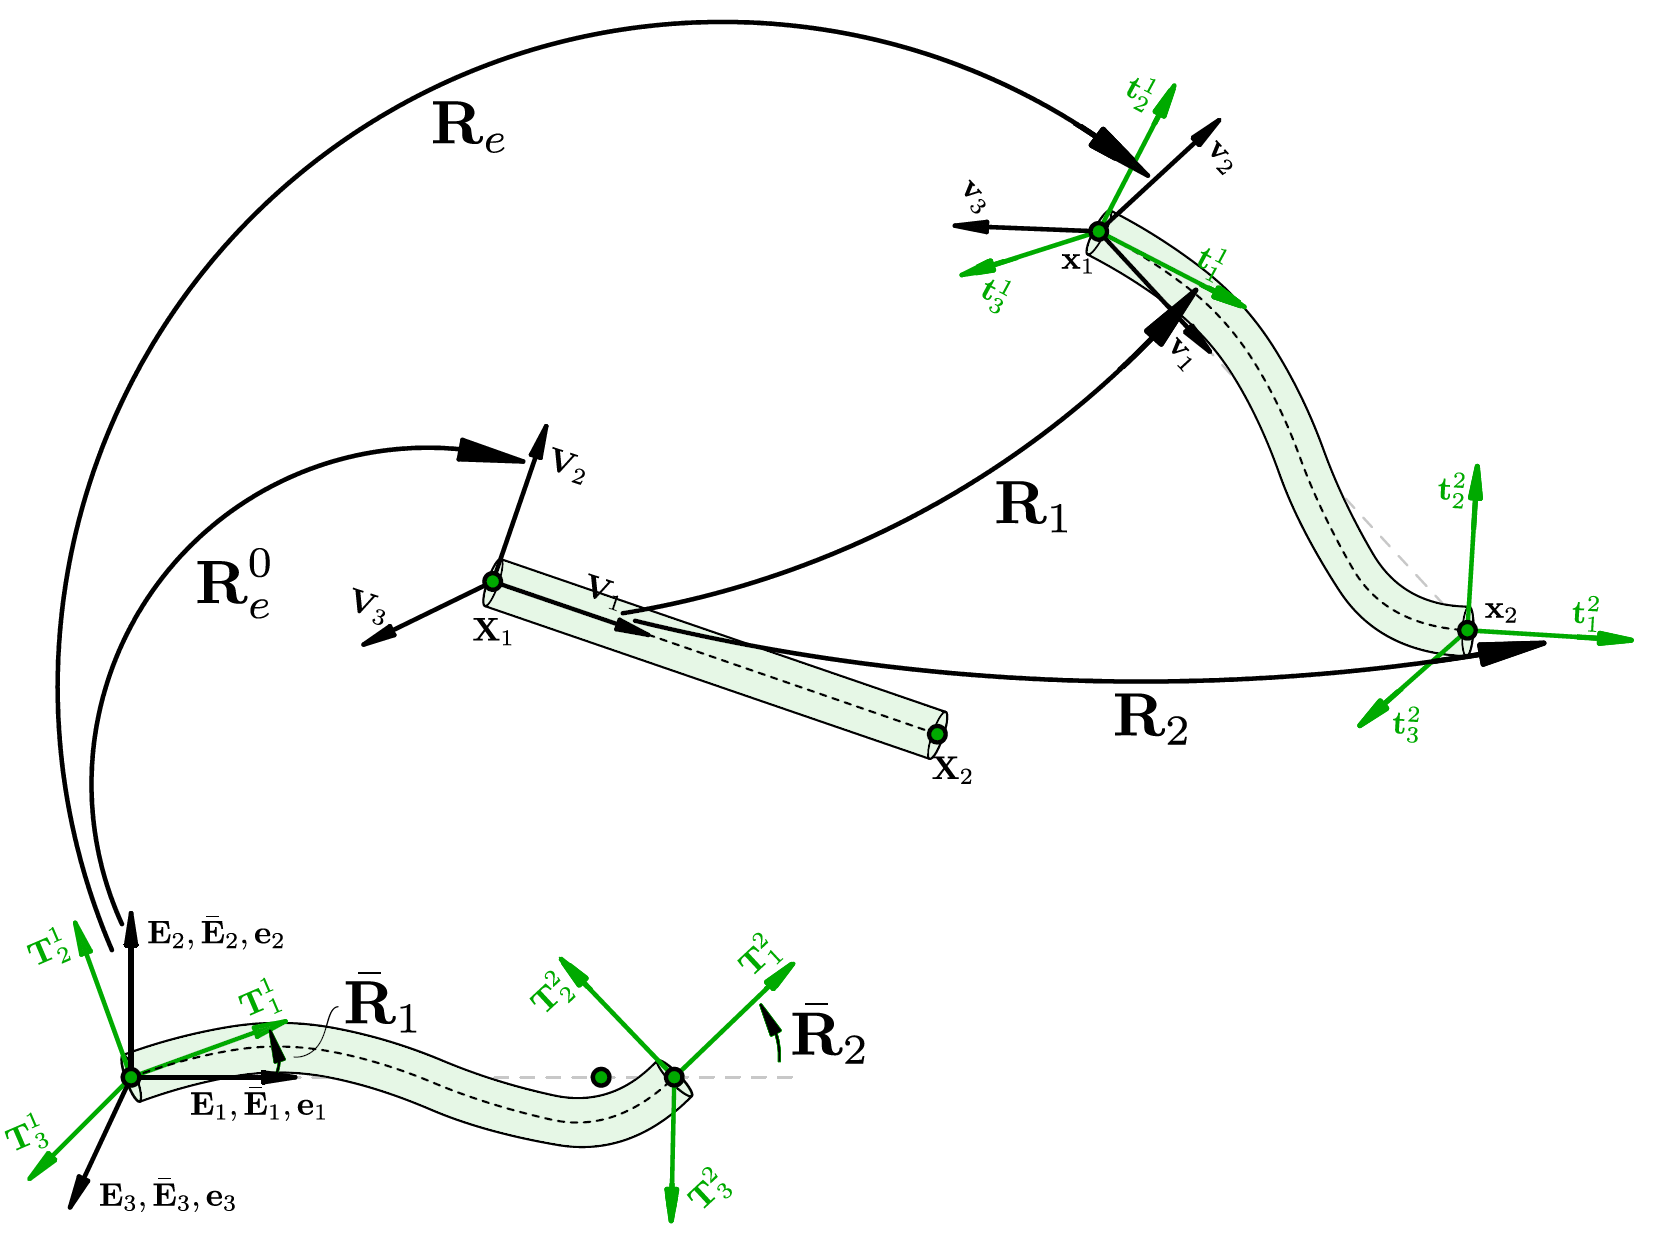
\includegraphics[width=.6\textwidth]{figures/configurations.png}
	\caption{Co-rotational element}
	\label{fig:corotational-config}
\end{figure}

\section{Regularized contact formulation}
The contact formulation presented in \cite{Aguirre2020}, is briefly presented in this section. In order to consider the contact against a rigid surface, the weak form  is extended using the variation of a penalty potential $\delta W_c$ as
\begin{align}
	\delta W=\delta W_{int} + \delta W_{kin} - \delta W_{ext} -\delta W_c= 0.\label{eq:deltaW-contact}
\end{align}
\noindent Following \cite{Wriggers2006}, a penalty potential is defined. This potential takes into account the normal and frictional contributions of the beam contact against a rigid master surface $\Gamma_s$
\begin{align}
	\delta W_c = \int_0^{l_0}\left(p_N\delta g_N+\vect{t}_T\cdot\delta\vect{g}_T\right)\,ds,\label{eq:deltWc-friction}
\end{align}
\noindent with $g_N$ being the normal gap respect the master surface, $\vect{g}_T$ the relative displacement in the tangential direction, $p_N$ the contact pressure and $\vect{t}_T$ the frictional contact traction.  All values in (\ref{eq:deltWc-friction}) are evaluated at the beam centerline by assuming that the beam radius is small enough to disregard the couples generated by the frictional force \cite{Zavarise2000}. Given the fact that circular beams are used,  $g_N$ is defined as
\begin{align}
		g_N(s) = d_s (s) -  r,\label{eq:gN}
\end{align}

\noindent with $d_{s}(s)$ being the distance of a point on the beam centerline to the surface and $r$ the radius of the beam, which is assumed constant. The variation of $g_N$ is given by
\begin{align}
	\delta g_N = \frac{\partial g_N}{\partial\vect{x}}\cdot\delta\vect{x}_0 = \frac{\partial d_{\Gamma_s}}{\partial\vect{x}}\cdot\delta\vect{u}_0 = \vect{n}\cdot\delta\vect{u}_0,\label{eq:delta-gN}
\end{align}
\noindent with $\vect{n}$ being the surface normal. In order to obtain the variation of $\vect{g}_T$, the centerline displacement is decomposed into its normal and tangential components, respect to the master surface \cite{Ortega2017}, i.e.
\begin{align}
	\delta\vect{u}_0 = \left(\delta\vect{u}_0\cdot\vect{n}\right)\vect{n} + \delta\vect{u}_T = \delta g_N\frac{\partial g_N}{\partial\vect{x}}+\delta\vect{g}_T.
\end{align}
\noindent Isolating $\delta\vect{g}_T$ in the above expression yields
\begin{align}
	\delta\vect{g}_T =\left(\vect{I}-\frac{\partial g_N}{\partial\vect{x}}\otimes\frac{\partial g_N}{\partial\vect{x}}\right)\delta\vect{u}_0,\label{eq:delta-gT}\\
	\dot{\vect{g}}_T = \left(\vect{I}-\frac{\partial g_N}{\partial\vect{x}}\otimes\frac{\partial g_N}{\partial\vect{x}}\right)\dot{\vect{u}}_0.
\end{align}

In order to facilitate the convergence of the Newton Raphson algorithm, both the contact pressure $p_N$ and frictional contact force $\vect{t}_T$ are regularized. The contact pressure is evaluated using the penalty regularization used in \cite{Durville2012,Meier2016,Meier2017,Meier2017b}
\begin{align}
	p_N^{reg} &= \left\{\begin{array}{ll}
		\bar{p}_N-\varepsilon_c g_N,&g\leq 0\\
		&\\
		\dfrac{\varepsilon_c\bar{g}_N-\bar{p}_N}{\bar{g}_N^2}g_N^2-\varepsilon_c g_N + 
		\bar{p}_N,&0<g_N\leq \bar{g}_N\\
		&\\
		0,&g>\bar{g}_N
	\end{array}\right.\label{eq:pN}
\end{align}
\noindent with $\varepsilon_c$ being the penalty parameter, $\bar{p}_N=\frac{1}{2}\varepsilon_c\bar{g}_N$ and $\bar{g}_N$ being the normal gap value at which the contact pressure starts increasing. As in \cite{Meier2017}, $\bar{g}_N$ is taken as 10\% of the beam radius. 

The discrete contact force vector is defined as

\begin{align}
	\vect{T}_c = \int_0^{l_0}\vect{E}\vect{H}^T_1\vect{R}_e^T\vect{f}_c\,ds,\label{eq:Tc}
\end{align}


\noindent  with $\vect{f}_c$ being the contact force, given by
\begin{align}
	\vect{f}_c = \vect{f}_c^N + \vect{f}_c^T\label{eq:fc-1},
\end{align}

\noindent with
\begin{align}
	\vect{f}_c^N &= p_N^{reg}\frac{\partial g_N}{\partial\vect{x}},\label{eq:fcN}\\
	\vect{f}_c^T&=-\mu p_N^{reg}\frac{\dot{\vect{g}}_T^h}{\sqrt{\|\dot{\vect{g}}_T^h\|^2+\varepsilon}}.\label{eq:fcT}
\end{align}


\section{Hybrid stick-slip formulation as in \cite{Geilinger2020}}
We briefly describe the formulation presented in \cite{Geilinger2020}, but adapted to our notation. The normal and tangential components in \ref{eq:fc-1} are given by 
\begin{align}
	\vect{f}_c^N &= p_N^{lin}\frac{\partial g_N}{\partial\vect{x}},\label{eq:fcN-Geilinger}\\
	\vect{f}_c^T&=- \frac{\dot{\vect{g}}_T^h}{\|\dot{\vect{g}}_T^h\|}\min\left(\varepsilon_c^T\|\dot{\vect{g}}_T\|,\mu p_N^{lin}\right),\label{eq:fcT-Geilinger}
\end{align}
\noindent with
\begin{align}
	p_N^{lin} = \varepsilon_c^N\max (-g_N,0).
\end{align}
\noindent \textbf{Note}:  the regularized normal pressure is no longer used. They claim that in very few instances the Gauss Point falls into $g_N=0$, which is the only point with a non-defined derivative. 


\noindent \textbf{Note}: now two penalty parameters are defined, $\varepsilon_c^N$ and $\varepsilon_c^T$, but $\varepsilon_c^T$ is defined as $\varepsilon_c^T = \Delta t \varepsilon_c^N$ (see last paragraph of section 4.2 in \cite{Geilinger2020}). 

\noindent \textbf{Note}: restricting to the slip case, replacing $p_N^{lin}$ by $p_N^{reg}$ equations (\ref{eq:fcN-Geilinger}), (\ref{eq:fcT-Geilinger}) turn into equations (\ref{eq:fcN}), (\ref{eq:fcT}) for the specific case of $\varepsilon=0$.

\begin{figure}[!htbp]
	\centering
	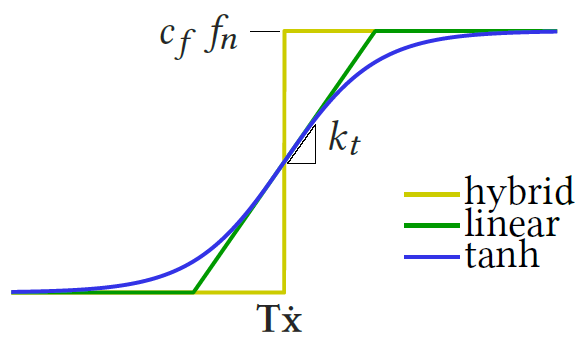
\includegraphics[width=.3\textwidth]{figures/friction_law.png}
	\caption{Friction law taken from \cite{Geilinger2020}}
	\label{fig:friction-law}
\end{figure}

The use of the above equations would yield to a linearaly regularized friction law, which does not account for stick (see Figure \ref{fig:friction-law}), which does not avoid long-term sliding. The hybrid algorithm proposed in \cite{Geilinger2020} is proposed to actually enforce stick. This is done by using the following algorithm:
\newpage
\begin{itemize}
	\item while $\|\vect{R}\|<\epsilon_R^{1/2}$, repeat at each iteration $k$
	\begin{itemize}
		\item solve system (\ref{eq:residual-algebraic}) using definitions (\ref{eq:fcN-Geilinger}) and (\ref{eq:fcT-Geilinger}) for the contact force
	\end{itemize}
	\item $\forall$ nodes compute $\vect{f}_c^T$ as defined in equation (\ref{eq:fcT-Geilinger}) and check Coulomb limit:
	\begin{itemize}
		\item if $\|\vect{f}_c^T\|<\mu p_N^{lin}$ $\rightarrow$ stick $\rightarrow$ apply fixed Dirichlet boundary conditions
		\item if $\|\vect{f}_c^T\|=\mu p_N^{lin}$ $\rightarrow$ slip $\rightarrow$ leave node free 
	\end{itemize}
	\item while $\|\vect{R}\|<\epsilon_R$, repeat at each iteration $k$
	\begin{itemize}
		\item solve system (\ref{eq:residual-algebraic}) using definitions (\ref{eq:fcN-Geilinger}) and (\ref{eq:fcT-Geilinger}) for the contact force
		\begin{itemize}
			\item $\forall$ \textbf{fixed nodes} compute $\vect{f}_c^T$ as defined in equation (\ref{eq:fcT-Geilinger}) and check Coulomb limit:
			\begin{itemize}
				\item if $\left(\|\vect{f}_c^T\|>\mu p_N^{lin}\right)$ \& $(\|\vect{R}\|<\epsilon_R^{1/2})$ $\rightarrow$ free that node
			\end{itemize}	
		\end{itemize}	
	\end{itemize}
\end{itemize}


\noindent \textbf{Note}: this algorithm has been written based on the description of  section 4.3 in \cite{Geilinger2020}. There are some parts that are not fully clear. Specifically: 1) if the fixed node is let free, can it be fixed again if the frictional force is below the Coulomb limit? My understanding is that everything is kept like this till the end of the simulation 2) using equation (\ref{eq:fcT-Geilinger}), the frictional force cannot be larger than $\mu p_N^{lin}$, therefore the $>$ symbol in the last check should be replaced by $=$? This would not make any difference, but I just wonder if I missed something in the description
\noindent 

\noindent \textbf{Note}: in our case, the frictional force is calculated at the Gauss points, whereas we can only fix nodes (not Gauss points). We should think of a way of transferring information from Gauss points to nodes or viceversa. Otherwise, we can check the Coulomb law at nodes and fix them if needed. The actual force we can keep using them at the 

\noindent \textbf{Note}: notice that, as explained in \cite{Geilinger2020}, the last check can lead to some nodes using the penalty frictional law, therefore sliding below the Coulomb limit. Apparently, this is very rare and has minor effects.
\newpage

\subsection{Proposed hybrid stick-slip}
Let's propose a very simple implementation where we keep almost all ingredients that we have, including the regularized laws for both normal contact and friction. I belive that we can still use them as they are just more general than the linear laws that they use, and what actually matters is that we check the Coulomb limit to enforce Dirichlet boundary conditions \textcolor{red}{(in red modifications respect to formulation in \cite{Geilinger2020})}. 

\vspace{5 mm}
\textcolor{red}{Initialize $\text{\textbf{f}}_c^T$, $\text{\textbf{p}}_N$ nodal vectors, of size ($3n_{nodes} \times 1$) and ($n_{nodes} \times 1$) respectively}

\begin{itemize}
	\item while $\|\vect{R}\|<\epsilon_R^{1/2}$, repeat at each iteration $k$
	\begin{itemize}
		\item \textcolor{red}{set $\text{\textbf{f}}_c^T(:)=0$, $\text{\textbf{f}}_c^N(:)=0$}
		\item solve system (\ref{eq:residual-algebraic}) \textcolor{red}{using definitions (\ref{eq:fcN}) and (\ref{eq:fcT}) for the contact force at each Gauss Point, integrated then into $\vect{T}_c$ as in equation (\ref{eq:Tc}) and assembled into the global $\text{\textbf{T}}_c$ vector}.
		\item \textcolor{red}{compute $\vect{f}_{c,elem}^T=\frac{1}{l_0}\int_0^{l_0}\vect{f}_{c}^T\,ds$, $p_N^{elem}=\frac{1}{l_0}\int_0^{l_0}p_N^{reg}\,ds$ and assemble $1/2$ of each term to the corresponding positions of nodes 1 and 2 in the nodal vectors $\text{\textbf{f}}_c^T$, $\text{\textbf{p}}_N$.}
	\end{itemize}
	\item \textcolor{red}{$\forall$ node i and using $\text{\textbf{f}}_c^T$, $\text{\textbf{p}}_N$, compare $\vect{f}_{c,i}^T$ to $p_{N,i}$}
	\begin{itemize}
		\item if $\|\vect{f}_{c,i}^T\|<\mu p_{N,i}$ $\rightarrow$ stick $\rightarrow$ apply fixed Dirichlet boundary conditions
		\item if $\|\vect{f}_{c,i}^T\|=\mu p_{N,i}$ $\rightarrow$ slip $\rightarrow$ leave node free 
	\end{itemize}
	\item while $\|\vect{R}\|<\epsilon_R$, repeat at each iteration $k$
	\begin{itemize}
		\item \textcolor{red}{set $\text{\textbf{f}}_c^T(:)=0$, $\text{\textbf{f}}_c^N(:)=0$}
		\item solve system (\ref{eq:residual-algebraic}) \textcolor{red}{using definitions (\ref{eq:fcN}) and (\ref{eq:fcT}) for the contact force at each Gauss Point, integrated then into $\vect{T}_c$ as in equation (\ref{eq:Tc}) and assembled into the global $\text{\textbf{T}}_c$ vector}.
		\item \textcolor{red}{compute $\vect{f}_{c,elem}^T=\frac{1}{l_0}\int_0^{l_0}\vect{f}_{c}^T\,ds$, $p_N^{elem}=\frac{1}{l_0}\int_0^{l_0}p_N^{reg}\,ds$ and assemble $1/2$ of each term to the corresponding positions of nodes 1 and 2 in the nodal vectors $\text{\textbf{f}}_c^T$, $\text{\textbf{p}}_N$.}
		\begin{itemize}
			\item $\forall$ \textbf{fixed nodes} \textcolor{red}{i and using $\text{\textbf{f}}_c^T$, $\text{\textbf{p}}_N$, compare $\vect{f}_{c,i}^T$ to $p_{N,i}$}
			\begin{itemize}
				\item if $\left(\|\vect{f}_{c,i}^T\|>\mu p_{N,i}\right)$ \& $(\|\vect{R}\|<\epsilon_R^{1/2})$ $\rightarrow$ free that node
			\end{itemize}	
		\end{itemize}	
	\end{itemize}
\end{itemize}
\newpage
\section{Alternative stick-slip}
The contact force vector is defined as
\begin{align}
	\vect{T}_c = \int_0^{l_0}\vect{E}\vect{H}^T_1\vect{R}_e^T\vect{f}_c\,ds,
\end{align}
\noindent with $\vect{f}_c$ defined as
\begin{align}
	\vect{f}_c = \vect{f}_N + \vect{f}_T;\qquad \vect{f}_N =p_N(\vect{d})\frac{\partial g_N}{\partial\vect{x}}\label{eq:fc}
\end{align}

\noindent and with $\vect{f}_T$ that can change between two different states:

\begin{align}
\vect{f}_T = \left\{\begin{array}{ll}
	-k_t\delta_t\frac{\dot{\vect{g}}_T^h}{\sqrt{\|\dot{\vect{g}}_T^h\|^2+\varepsilon}}-\eta_t\dot{\vect{g}}_T^h,&\text{if }\|\dot{\vect{g}}_T^h\| < v_s\text{ AND }\left\Vert-k_t\delta_t\frac{\dot{\vect{g}}_T^h}{\sqrt{\|\dot{\vect{g}}_T^h\|^2+\varepsilon}}-\eta_t\dot{\vect{g}}_T^h\right\Vert\leq \mu_{stick}p_N\\
	&\\
	-\mu_{slip} p_N\frac{\dot{\vect{g}}_T^h}{\sqrt{\|\dot{\vect{g}}_T^h\|^2+\varepsilon}},&\text{if }\|\dot{\vect{g}}_T^h\| \geq v_s
\end{array}\right.
\end{align}

In the transtion from dynamic to static contact, the initial guess for $\delta_t$ can be given by:

\begin{align}
	\delta_t = \frac{\mu_{slip}p_N}{k_t}-\frac{\eta_t}{k_t}\sqrt{\|\dot{\vect{g}}_T^h\|^2+\varepsilon}.
\end{align}

The linearization of the above contact force is computed as follows.
\begin{align}
	\delta\vect{T}_c = \vect{K}_c\delta\vect{d}+\vect{C}_c\delta\dot{\vect{d}};\quad\vect{K}_c = \vect{K}_c^1+\vect{K}_c^2+\vect{K}_c^3+\vect{K}_c^4.\label{eq:deltaTc-app}
\end{align}

 The following abbreviations are used (see for example \cite{Meier2017a})
\begin{subequations}
	\begin{align}
		&\vect{K}_c^1\delta\vect{d}=\int_0^{l_0}\vect{t}_c^1,ds,\label{eq:Kc1}\\
		&\vect{K}_c^2\delta\vect{d}=\int_0^{l_0}\vect{t}_c^2\,ds,\label{eq:Kc2}\\
		&\vect{K}_c^3\delta\vect{d}=\int_0^{l_0}\vect{t}_c^3\,ds,\label{eq:Kc3}\\
		&\vect{K}_c^4\delta\vect{d}+\vect{C}_c\delta\dot{\vect{d}}=\int_0^{l_0}\vect{t}_c^4\,ds,\label{eq:Kc4}
	\end{align}\label{eq:Kci}
\end{subequations}
\noindent with
\begin{subequations}
	\begin{align}
		\vect{t}_c^1&=\delta\vect{E}\vect{H}^T_1\vect{R}_e^T\vect{f}_c,\\
		\vect{t}_c^2&=\vect{E}(\delta\vect{H}_1)^T\vect{R}_e^T\vect{f}_c,\\
		\vect{t}_c^3&=\vect{E}\vect{H}_1^T(\delta\vect{R}_e)^T\vect{f}_c,\\
		\vect{t}_c^4&=\vect{E}\vect{H}_1^T\vect{R}_e^T\delta\vect{f}_c.
	\end{align}\label{eq:tci-intro}
\end{subequations}
\noindent Before moving forward with the above linearizations, it is useful to provide some preliminary results. Firstly, $\vect{f}_c$ is rigidly rotated back to give
\begin{align}
	\vect{\mathcal{F}}_c = \vect{R}_e^T\vect{f}_c\label{eq:Fc}.
\end{align}
\noindent At the same time the operator $\hat{\vect{S}}(\cdot)$ is defined, which transforms a $12\times 1$ array $\vect{a}$ into a $12\times 3$ matrix $\vect{A}$ as
\begin{align}
	\vect{A}=\hat{\vect{S}}(\vect{a}) &= \left[\begin{array}{c}
		\vect{S}(\vect{a}_1)\\\vect{S}(\vect{a}_2)\\\vect{S}(\vect{a}_3)\\\vect{S}(\vect{a}_4 )
	\end{array}\right];\quad \vect{a}_I = \left[\begin{array}{c}
		a_{3(I-1)+1}\\a_{3(I-1)+2}\\a_{3(I-1)+3}
	\end{array}\right];\quad I \in \{1,2,3,4\},\label{eq:Shat}
\end{align}
\noindent with the operator $\vect{S}$ as defined in equation (\ref{eq:S-psi}). 

In order to obtain $\vect{t}_c^1$, the variation $\delta\vect{E}$ is needed. This can be obtained from its definition (\ref{eq:deltaD-deltad}) and equation (\ref{eq:delta-Re-2}), to give
\begin{align}
	\delta\vect{E}&=\vect{E}\left[\begin{array}{cccc}
		\vect{S}(\delta\vect{W}_e) &\vect{0} &\vect{0} &\vect{0}\\
		\vect{0} &\vect{S}(\delta\vect{W}_e) &\vect{0} &\vect{0}\\
		\vect{0} & \vect{0} &\vect{S}(\delta\vect{W}_e) &\vect{0}\\
		\vect{0} & \vect{0} &\vect{0} &\vect{S}(\delta\vect{W}_e)
	\end{array}\right].\label{eq:deltaE}
\end{align}

\noindent And, in order to obtain $\vect{t}_{c}^4$, the variation of $\delta\vect{f}_c$ is needed. From equation (\ref{eq:fc}) this can be obtained as
\begin{align}
	\delta\vect{f}_c =\delta\vect{f}_N + \delta\vect{f}_T\label{eq:deltafc},
\end{align}
\noindent  The variation of $\vect{f}_N$ depends only on $\delta\vect{d}$ and is given as
\begin{align}
	\delta \vect{f}_N  =  p_N'(g_N)  \left(\frac{\partial g_N}{\partial\vect{x}}\otimes\frac{\partial g_N}{\partial\vect{x}}\right)\vect{R}_e\vect{H}_1\vect{E}^T\delta\vect{d}+p_N\frac{\partial^2g_N}{\partial\vect{x}\partial\vect{x}}\vect{R}_e\vect{H}_1\vect{E}^T\delta\vect{d},\label{eq:deltapN}
\end{align}
\noindent with $p_N'$ obtained from (\ref{eq:pN})
\begin{align}
	p_N' &= p_N'(g_N)=\left\{\begin{array}{ll}
		-\varepsilon_c ,&g\leq 0\\
		&\\
		2\dfrac{\varepsilon_c\bar{g}_N-\bar{p}_N}{\bar{g}_N^2}g_N-\varepsilon_c ,&0<g_N\leq \bar{g}_N\\
		&\\
		0.&g>\bar{g}_N
	\end{array}\right.\label{eq:pNprime}
\end{align}
The variation of $\vect{f}_T$ requires 
\begin{align}
	\delta\left(\frac{\dot{\vect{g}}_T^h}{\sqrt{\|\dot{\vect{g}}_T^h\|^2+\varepsilon}}\right)&=\frac{1}{\sqrt{\|\dot{\vect{g}}_T^h\|^2+\varepsilon}}\left(\vect{I}-\frac{1}{\|\dot{\vect{g}}_T^h\|^2+\varepsilon}(\dot{\vect{g}}_T^h\otimes\dot{\vect{g}}_T^h)\right)\delta\dot{\vect{g}}_T^h,\label{eq:delta_normalized_vector}
\end{align}

\noindent and the variation $\delta\dot{\vect{g}}_T^h$, which is given by
\begin{align}
	\delta\dot{\vect{g}}_T^h=\vect{\mathcal{A}}\delta\vect{d}+\vect{\mathcal{B}}\delta\dot{\vect{d}};\quad\vect{\mathcal{A}}=\vect{\mathcal{A}}^1+\vect{\mathcal{A}}^2+\vect{\mathcal{A}}^3+\vect{\mathcal{A}}^4\label{eq:deltagdot},
\end{align}
\noindent with
\begin{subequations}
	\begin{align}
		\vect{\mathcal{A}}^1=&-\left(\frac{\partial g_N}{\partial\vect{x}}\cdot(\vect{R}_e\vect{H}_1\dot{\vect{\mathcal{D}}})\right)\frac{\partial^2 g_N}{\partial\vect{x}\partial\vect{x}}\vect{R}_e\vect{H}_1\vect{E}^T\nonumber\\
		&-\frac{\partial g_N }{\partial\vect{x}}\otimes\left(\vect{E}\vect{H}_1^T\vect{R}_e^T\frac{\partial^2 g_N}{\partial\vect{x}\partial\vect{x}}\vect{R}_e\vect{H}_1\dot{\vect{\mathcal{D}}}\right),\\
		\vect{\mathcal{A}}^2=&-\left(\vect{I}-\frac{\partial g_N}{\partial\vect{x}}\otimes\frac{\partial g_N}{\partial\vect{x}}\right)\vect{R}_e\vect{S}(\vect{H}_1\dot{\vect{\mathcal{D}}})\vect{G}^T\vect{E}^T,\\
		\vect{\mathcal{A}}^3=&\left(\vect{I}-\frac{\partial g_N}{\partial\vect{x}}\otimes\frac{\partial g_N}{\partial\vect{x}}\right)\left(\frac{N_7}{l_n^2}\vect{R}_e\vect{A}_1\dot{\vect{\mathcal{D}}}\vect{r}+\vect{R}_e\vect{S}(\vect{G}^T\dot{\vect{\mathcal{D}}})\vect{P}_1\vect{P}\vect{E}^T\right),\\
		\vect{\mathcal{A}}^4=&\left(\vect{I}-\frac{\partial g_N}{\partial\vect{x}}\otimes\frac{\partial g_N}{\partial\vect{x}}\right)\vect{R}_e\vect{H}_1\hat{\vect{S}}(\dot{\vect{\mathcal{D}}})\vect{G}^T\vect{E}^T,\\
		\vect{\mathcal{B}}=&\left(\vect{I}-\frac{\partial g_N}{\partial\vect{x}}\otimes\frac{\partial g_N}{\partial\vect{x}}\right)\vect{R}_e\vect{H}_1\vect{E}^T.
	\end{align}
\end{subequations}

These results allow computing the variation of the tangential contact force. We write it seperately for the stick and slip case.

\noindent\textbf{Stick}:
\begin{align}
	\delta\vect{f}_T&=-k_t\delta_t\delta\left(\frac{\dot{\vect{g}}_T^h}{\sqrt{\|\dot{\vect{g}}_T^h\|^2+\varepsilon}}\right)-\eta_t\delta\dot{\vect{g}}_T^h\\
	&=-k_t\delta_t\left(\frac{1}{\sqrt{\|\dot{\vect{g}}_T^h\|^2+\varepsilon}}\left(\vect{I}-\frac{1}{\|\dot{\vect{g}}_T^h\|^2+\varepsilon}(\dot{\vect{g}}_T^h\otimes\dot{\vect{g}}_T^h)\right)\delta\dot{\vect{g}}_T^h\right)-\eta_t\delta\dot{\vect{g}}_T^h\\
	&=-\left(\frac{k_t\delta_t}{\sqrt{\|\dot{\vect{g}}_T^h\|^2+\varepsilon}}\left(\vect{I}-\frac{1}{\|\dot{\vect{g}}_T^h\|^2+\varepsilon}(\dot{\vect{g}}_T^h\otimes\dot{\vect{g}}_T^h)\right)+\eta_t\vect{I}\right)\left(\vect{\mathcal{A}}\delta\vect{d}+\vect{\mathcal{B}}\delta\dot{\vect{d}}\right).
\end{align}

\noindent\textbf{Slip}:
\begin{align}
	\delta\vect{f}_T=&\delta\left(-\mu_{slip} p_N\frac{\dot{\vect{g}}_T^h}{\sqrt{\|\dot{\vect{g}}_T^h\|^2+\varepsilon}}\right)\\
	=&-\frac{\mu_{slip}}{\sqrt{\|\dot{\vect{g}}_T^h\|^2+\varepsilon}}p_N'(g_N)\left(\dot{\vect{g}}_T^h\otimes\frac{\partial g_N}{\partial\vect{x}}\right)\vect{R}_e\vect{H}_1\vect{E}^T\delta\vect{d}\\
	&-\frac{\mu_{slip}}{\sqrt{\|\dot{\vect{g}}_T^h\|^2+\varepsilon}}p_N(g_N)\left(\vect{I}-\frac{1}{\|\dot{\vect{g}}_T^h\|^2+\varepsilon}(\dot{\vect{g}}_T^h\otimes\dot{\vect{g}}_T^h)\right)\left(\vect{\mathcal{A}}\delta\vect{d}+\vect{\mathcal{B}}\delta\dot{\vect{d}}\right).
\end{align}

\noindent Using the above results yields
\begin{align}
	\delta\vect{f}_c =\vect{K}_{\vect{f}_c}\delta\vect{d}+\vect{C}_{\vect{f}_c}\delta\dot{\vect{d}},\label{eq:deltafc-2}
\end{align}
\noindent with
\begin{align}
	\vect{K}_{\vect{f}_c}&=\vect{K}_{\vect{f}_N}+\vect{K}_{\vect{f}_T},\\
	\vect{C}_{\vect{f}_c}&=\vect{C}_{\vect{f}_T}.
\end{align}
The normal component matrices are computed as
\begin{align}
	\vect{K}_{\vect{f}_N} &=   \left( p_N'(g_N)\left(\frac{\partial g_N}{\partial\vect{x}}\otimes\frac{\partial g_N}{\partial\vect{x}}\right)+p_N\frac{\partial^2g_N}{\partial\vect{x}\partial\vect{x}}\right)\vect{R}_e\vect{H}_1\vect{E}^T.
\end{align}

For the tangential component, we decompose into stick and slip

\noindent\textbf{Stick}:
\begin{align}
	\vect{K}_{\vect{f}_T}&=-\left(\frac{k_t\delta_t}{\sqrt{\|\dot{\vect{g}}_T^h\|^2+\varepsilon}}\left(\vect{I}-\frac{1}{\|\dot{\vect{g}}_T^h\|^2+\varepsilon}(\dot{\vect{g}}_T^h\otimes\dot{\vect{g}}_T^h)\right)+\eta_t\vect{I}\right)\vect{\mathcal{A}},\\
	\vect{C}_{\vect{f}_T}&=-\left(\frac{k_t\delta_t}{\sqrt{\|\dot{\vect{g}}_T^h\|^2+\varepsilon}}\left(\vect{I}-\frac{1}{\|\dot{\vect{g}}_T^h\|^2+\varepsilon}(\dot{\vect{g}}_T^h\otimes\dot{\vect{g}}_T^h)\right)+\eta_t\vect{I}\right)\vect{\mathcal{B}}.
\end{align}

\noindent\textbf{Slip}:
\begin{align}
	\vect{K}_{\vect{f}_T}=&-\frac{\mu_{slip}}{\sqrt{\|\dot{\vect{g}}_T^h\|^2+\varepsilon}}p_N'(g_N)\left(\dot{\vect{g}}_T^h\otimes\frac{\partial g_N}{\partial\vect{x}}\right)\vect{R}_e\vect{H}_1\vect{E}^T\\
	&-\frac{\mu_{slip}}{\sqrt{\|\dot{\vect{g}}_T^h\|^2+\varepsilon}}p_N(g_N)\left(\vect{I}-\frac{1}{\|\dot{\vect{g}}_T^h\|^2+\varepsilon}(\dot{\vect{g}}_T^h\otimes\dot{\vect{g}}_T^h)\right)\vect{\mathcal{A}},\\
	\vect{C}_{\vect{f}_T}=&-\frac{\mu_{slip}}{\sqrt{\|\dot{\vect{g}}_T^h\|^2+\varepsilon}}p_N(g_N)\left(\vect{I}-\frac{1}{\|\dot{\vect{g}}_T^h\|^2+\varepsilon}(\dot{\vect{g}}_T^h\otimes\dot{\vect{g}}_T^h)\right)\vect{\mathcal{B}}.
\end{align}

\noindent With all the information above we can finally assemble the elemental matrices. Using (\ref{eq:Fc}), (\ref{eq:Shat}), (\ref{eq:deltaE}), (\ref{eq:deltafc-2}) gives
\begin{subequations}
	\begin{align}
		\vect{t}_c^1&=\delta\vect{E}\vect{H}^T_1\vect{\mathcal{F}}_c=  \vect{E}\left[\begin{array}{c}
			\vect{S}(\delta\vect{W}_e)\left[\vect{H}^T_1\vect{\mathcal{F}}_c\right]_{1:3} \\
			\vect{S}(\delta\vect{W}_e)\left[\vect{H}^T_1\vect{\mathcal{F}}_c\right]_{4:6} \\
			\vect{S}(\delta\vect{W}_e)\left[\vect{H}^T_1\vect{\mathcal{F}}_c\right]_{7:9}\\
			\vect{S}(\delta\vect{W}_e)\left[\vect{H}^T_1\vect{\mathcal{F}}_c\right]_{10:12}
		\end{array}\right]\nonumber\\
		&=  -\vect{E}\hat{\vect{S}}(\vect{H}^T_1\vect{\mathcal{F}}_c)\delta\vect{W}_e= -\vect{E}\hat{\vect{S}}(\vect{H}^T_1\vect{\mathcal{F}}_c)\vect{G}^T\vect{E}^T\delta\vect{d},\label{eq:tc1}\\
		\vect{t}_c^2&=\vect{E}\delta\vect{H}_1^T\vect{\mathcal{F}}_c=\vect{E}\left(\frac{N_7}{l_n^2}\vect{A}_1\vect{r}\delta\vect{d}-\vect{S}(\delta\vect{u}_l^t)\vect{G}^T\right)^T\vect{\mathcal{F}}_c\nonumber\\ &=\frac{N_7}{l_n^2}\vect{E}\vect{A}_1^T\vect{\mathcal{F}}_c\left(\vect{r}\delta\vect{d}\right)+\vect{E}\vect{G}\vect{S}(\delta\vect{u}^t)\vect{\mathcal{F}}_c\nonumber\\
		&= \frac{N_7}{l_n^2}\vect{E}\vect{A}_1^T\vect{\mathcal{F}}_c\vect{r}\delta\vect{d}-\vect{E}\vect{G}\vect{S}(\vect{\mathcal{F}}_c)\vect{P}_1\vect{P}\vect{E}^T\delta\vect{d},\label{eq:tc2}\\
		\vect{t}_c^3&=\vect{E}\vect{H}_1^T(\delta\vect{R}_e)^T\vect{f}_c= \vect{E}\vect{H}_1^T\left(\vect{R}_e\vect{S}(\delta\vect{W}_e)\right)^T\vect{f}_c= -\vect{E}\vect{H}_1^T\vect{S}(\delta\vect{W}_e)\vect{\mathcal{F}}_c\nonumber\label{eq:tc3}\\
		&= \vect{E}\vect{H}_1^T\vect{S}(\vect{\mathcal{F}}_c)\delta\vect{W}_e=\vect{E}\vect{H}_1^T\vect{S}(\vect{\mathcal{F}}_c)\vect{G}^T\vect{E}^T\delta\vect{d},\\
		\vect{t}_c^4&=\vect{E}\vect{H}_1^T\vect{R}_e^T\delta\vect{f}_c=\vect{E}\vect{H}_1^T\vect{R}_e^T\left(\vect{K}_{\vect{f}_c}\delta\vect{d}+\vect{C}_{\vect{f}_c}\delta\dot{\vect{d}}\right).\label{eq:tc4}
	\end{align}\label{eq:tci}
\end{subequations}


\noindent Finally, using the results in (\ref{eq:tci}) into (\ref{eq:Kci}), the different tangent terms in (\ref{eq:deltaTc-app}) are given by
\begin{align}
	\vect{K}_c^1 &= -\int_0^{l_0}\vect{E}\hat{\vect{S}}(\vect{H}^T_1\vect{\mathcal{F}}_c)\vect{G}^T\vect{E}^T\,ds,\\
	\vect{K}_c^2 &=\int_0^{l_0} \left(\frac{N_7}{l_n^2}\vect{E}\vect{A}_1^T\vect{\mathcal{F}}_c\vect{r}-\vect{E}\vect{G}\vect{S}(\vect{\mathcal{F}}_c)\vect{P}_1\vect{P}\vect{E}^T\right)\,ds,\\
	\vect{K}_c^3 &=\int_0^{l_0} \vect{E}\vect{H}_1^T\vect{S}(\vect{\mathcal{F}}_c)\vect{G}^T\vect{E}^T\,ds,\\
	\vect{K}_c^4 &=\int_0^{l_0}\vect{E}\vect{H}_1^T\vect{R}_e^T\vect{K}_{\vect{f}_c}\,ds,\\
	\vect{C}_c &=\int_0^{l_0}\vect{E}\vect{H}_1^T\vect{R}_e^T\vect{C}_{\vect{f}_c}\,ds.
\end{align}

\section{Adding damping to the normal contact}

In this section, we keep the same formulation as before, but we add a normal damping term. The normal force is redefined as (see equation (\ref{eq:fc}))
\begin{align}
\vect{f}_N =p_N(\vect{d})\frac{\partial g_N}{\partial\vect{x}}-\mu_{n}\dot{\vect{g}}_N^h;\quad \dot{\vect{g}}_N^h = \left(\dot{\vect{u}}_0^h\cdot\frac{\partial g_N}{\partial \vect{x}}\right)\frac{\partial g_N}{\partial \vect{x}}=\left(\frac{\partial g_N}{\partial \vect{x}}\otimes\frac{\partial g_N}{\partial \vect{x}}\right)\dot{\vect{u}}_0^h.
\end{align}
\noindent \textbf{Note}: we need to keep in mind that the above formulation, as written, adds normal damping even if there is no contact. If we force in the code that the damping is only activated when contact occurs (i.e. $p_N>0$), then we may have an abrupt change in $\vect{f}_N$. In any case, this is the simple derivation (and implementation), so it is worth trying this first.


To simplify the derivations, let's split the normal force into a displacement term $\vect{f}_N^\delta$ (the variation of which was derived in the previous section) and a viscous term $\vect{f}_N^v$, i.e.
\begin{align}
	\vect{f}_N = \vect{f}_N^\delta + \vect{f}_N^v;\quad \vect{f}_N^\delta = p_N\frac{\partial g_N}{\partial\vect{x}},\quad \vect{f}_N^v = -\mu_N^v\dot{\vect{g}}_N^h.
\end{align}

The variation of $\vect{f}_N^v$ requires the variation of $\dot{\vect{g}}_N^h$. Following the derivations fro the variation of $\dot{\vect{g}}_T^h$ from the previous section, we obtain
\begin{align}
	\delta\dot{\vect{g}}_N^h=\vect{\mathcal{A}}_N\delta\vect{d}+\vect{\mathcal{B}}_N\delta\dot{\vect{d}};\quad\vect{\mathcal{A}}_N=\vect{\mathcal{A}}_N^1+\vect{\mathcal{A}}_N^2+\vect{\mathcal{A}}_N^3+\vect{\mathcal{A}}_N^4\label{eq:deltagdotN},
\end{align}
\noindent with
\begin{subequations}
	\begin{align}
		\vect{\mathcal{A}}_N^1=&\left(\frac{\partial g_N}{\partial\vect{x}}\cdot(\vect{R}_e\vect{H}_1\dot{\vect{\mathcal{D}}})\right)\frac{\partial^2 g_N}{\partial\vect{x}\partial\vect{x}}\vect{R}_e\vect{H}_1\vect{E}^T\nonumber\\
		&\frac{\partial g_N }{\partial\vect{x}}\otimes\left(\vect{E}\vect{H}_1^T\vect{R}_e^T\frac{\partial^2 g_N}{\partial\vect{x}\partial\vect{x}}\vect{R}_e\vect{H}_1\dot{\vect{\mathcal{D}}}\right),\\
		\vect{\mathcal{A}}_N^2=&-\left(\frac{\partial g_N}{\partial\vect{x}}\otimes\frac{\partial g_N}{\partial\vect{x}}\right)\vect{R}_e\vect{S}(\vect{H}_1\dot{\vect{\mathcal{D}}})\vect{G}^T\vect{E}^T,\\
		\vect{\mathcal{A}}_N^3=&\left(\frac{\partial g_N}{\partial\vect{x}}\otimes\frac{\partial g_N}{\partial\vect{x}}\right)\left(\frac{N_7}{l_n^2}\vect{R}_e\vect{A}_1\dot{\vect{\mathcal{D}}}\vect{r}+\vect{R}_e\vect{S}(\vect{G}^T\dot{\vect{\mathcal{D}}})\vect{P}_1\vect{P}\vect{E}^T\right),\\
		\vect{\mathcal{A}}_N^4=&\left(\frac{\partial g_N}{\partial\vect{x}}\otimes\frac{\partial g_N}{\partial\vect{x}}\right)\vect{R}_e\vect{H}_1\hat{\vect{S}}(\dot{\vect{\mathcal{D}}})\vect{G}^T\vect{E}^T,\\
		\vect{\mathcal{B}}_N=&\left(\frac{\partial g_N}{\partial\vect{x}}\otimes\frac{\partial g_N}{\partial\vect{x}}\right)\vect{R}_e\vect{H}_1\vect{E}^T.
	\end{align}
\end{subequations}
\noindent\textbf{Note}: if we end up using this formulation, we should simplify the above notation. One potential solution could be (for $\vect{\mathcal{A}}_N^4$, for example, but same for the other terms) to redefine the $\vect{\mathcal{A}}_4$ as $\vect{\mathcal{A}}_4=\vect{R}_e\vect{H}_1\hat{\vect{S}}(\dot{\vect{\mathcal{D}}})\vect{G}^T\vect{E}^T$. Then the contribution for the normal and tangential components would only differe by the premultiplication with, respectively, $\left(\frac{\partial g_N}{\partial\vect{x}}\otimes\frac{\partial g_N}{\partial\vect{x}}\right)$ and $\left(\vect{I}-\frac{\partial g_N}{\partial\vect{x}}\otimes\frac{\partial g_N}{\partial\vect{x}}\right)$. But let's stick for this notation for first implementation as otherwise it would be difficult to debug in case problems arise.

\noindent Using the above results yields (in red new or modified terms)
\begin{align}
	\delta\vect{f}_c =\textcolor{red}{\vect{K}_{\vect{f}_c}}\delta\vect{d}+\textcolor{red}{\vect{C}_{\vect{f}_c}}\delta\dot{\vect{d}},\label{eq:deltafc-2}
\end{align}
\noindent with
\begin{align}
	\vect{K}_{\vect{f}_c}&=\textcolor{red}{\vect{K}_{\vect{f}_N}}+\vect{K}_{\vect{f}_T},\\
	\vect{C}_{\vect{f}_c}&=\textcolor{red}{\vect{C}_{\vect{f}_N}}+\vect{C}_{\vect{f}_T}.
\end{align}
The normal component matrices are computed as
\begin{align}
	\textcolor{red}{\vect{K}_{\vect{f}_N}} &=   \left( p_N'(g_N)\left(\frac{\partial g_N}{\partial\vect{x}}\otimes\frac{\partial g_N}{\partial\vect{x}}\right)+p_N\frac{\partial^2g_N}{\partial\vect{x}\partial\vect{x}}\right)\vect{R}_e\vect{H}_1\vect{E}^T\textcolor{red}{-\mu_N^v\vect{\mathcal{A}}_N}\\
	\textcolor{red}{\vect{C}_{\vect{f}_N}} &=\textcolor{red}{-\mu_N^v\vect{\mathcal{B}}_N}.
\end{align}


%\bibliography{c:/Users/miquel/Dropbox/Feina/PhD/1.Work/2.Bibliography/thesis}
%\bibliography{D:/dropbox/Dropbox/Feina/library}
\newpage
%\textbf{References}
%\bibliography{C:/Users/miquel.aguirre/Dropbox/Feina/library}
\bibliographystyle{model1-num-names}
\bibliography{C:/Users/miquel.aguirre/Dropbox/Feina/library}



\end{document}
